\section{Scopo del progetto}
\begin{frame}
	\frametitle{Scopo del progetto}
	\begin{center}
	\begin{large}
		\textbf{Monolith}: Framework per la creazione di bolle interattive \\
		\vspace{1cm}
		\textbf{Demo}: Bolla esempio che usa Monolith
	\end{large}
	\end{center}
	
\end{frame}

\section{Copertura dei Requisiti}
\begin{frame}
	\frametitle{Copertura dei Requisiti}
	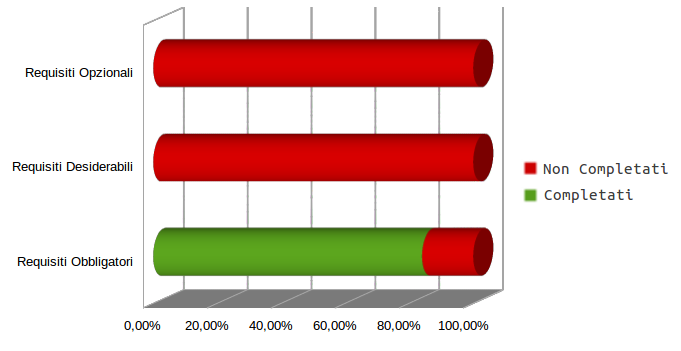
\includegraphics[scale=0.50]{img/Requisiti.png}
	
\end{frame}

\section{Nel prossimo periodo...}
\begin{frame}
	\frametitle{Nel prossimo periodo...}
	
	\begin{columns}
		\begin{column}{0.4\textwidth}
			
		\end{column}
		
		\begin{column}{0.5\textwidth}
			\begin{itemize}
				\begin{Large}
				\item Codice Demo
				\vspace{0.5cm}
				\item Manuali
				\vspace{0.5cm}
				\item Test
				\end{Large}		
			\end{itemize}
		\end{column}
		
		\begin{column}{0.2\textwidth}
			
		\end{column}
	\end{columns}
	
\end{frame}

\section{Test}

\subsection{Stato dei Test}
\begin{frame}
	\frametitle{Stato dei Test}
	\begin{center}
	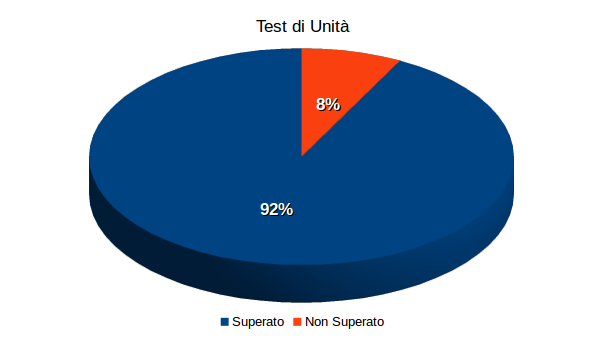
\includegraphics[scale=0.55]{img/TU.png}
	\end{center}
\end{frame}

\begin{frame}
	\frametitle{Stato dei Test}
	\begin{center}
	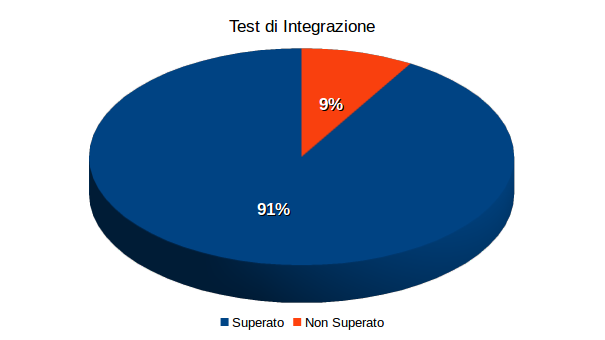
\includegraphics[scale=0.55]{img/TI.png}
    \end{center}
\end{frame}

\begin{frame}
	\frametitle{Stato dei Test}
	\begin{center}
	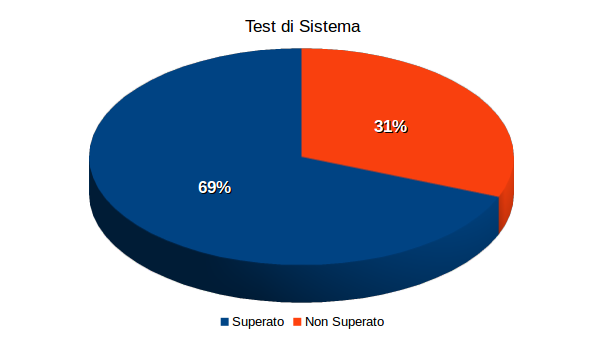
\includegraphics[scale=0.55]{img/TS.png}
    \end{center}
\end{frame}

\subsection{Strumenti usati}
\begin{frame}
	\frametitle{Strumenti usati}
	\begin{center}
	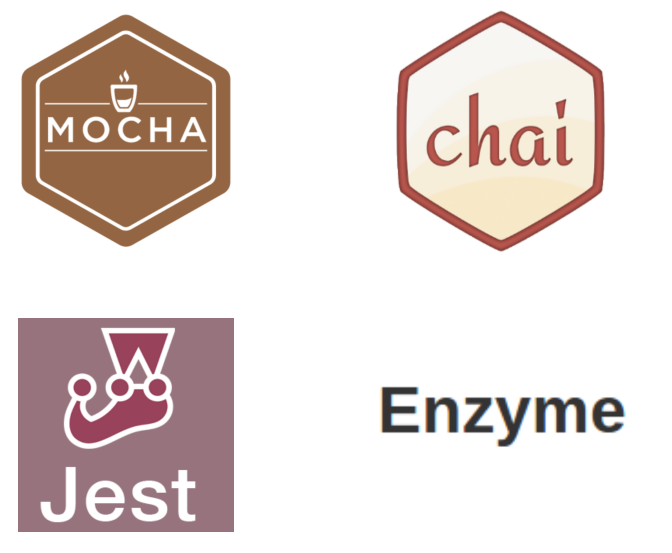
\includegraphics[scale=0.30]{img/strumenti.png}
	\end{center}
\end{frame}
